\documentclass{beamer}

\usepackage[english]{babel}
\usepackage[utf8x]{inputenc}
\usepackage[inline]{asymptote}
\usepackage{slide_helper}
\usepackage{tabu}

\usepackage{tikz}
\usetikzlibrary{arrows.meta}

\begin{asydef}
import graph;
import slopefield;
import fontsize;
defaultpen(fontsize(9pt));
ngraph=1000;

int pen_pos=-1;
pen[] pens={blue, red, heavycyan, heavymagenta, lightolive};
pens.cyclic=true;
pen next_color() {return pens[++pen_pos];}

DefaultHead.size=new real(pen p=currentpen) {return 2.5mm;};
\end{asydef}

\title[MA245 - Section 8.1]{Laplace Transforms}

\begin{document}

\begin{frame}
  \titlepage
\end{frame}

\begin{frame}
\begin{block}{}
In this chapter we shall study the Laplace transformation, which will allow us to reframe some types of hard problems \visible<2>{into equivalent easier problems.}
\end{block}
\begin{block}{}
\begin{center}
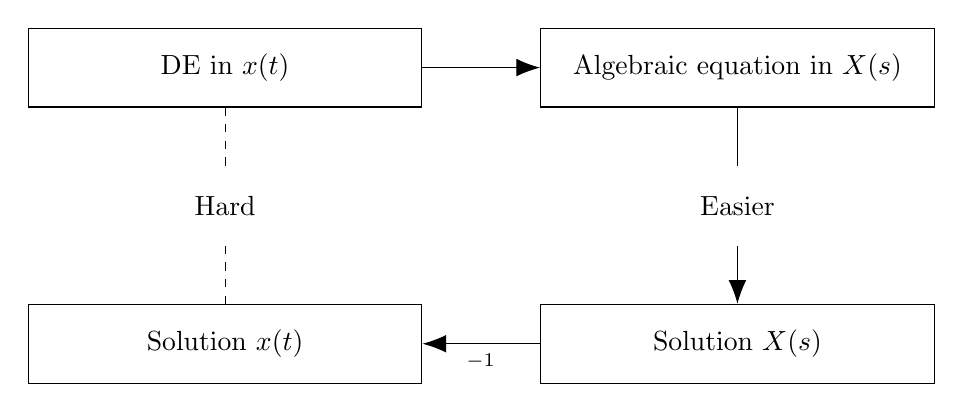
\begin{tikzpicture}
\node (DE) [draw,minimum width=5cm, minimum height=1cm] {DE in $x(t)$};
\node (DESol) [draw,minimum width=5cm, minimum height=1cm,yshift=-3cm] at (DE.south) {Solution $x(t)$};
\node (Hard) [dashed,minimum width=1cm,minimum height=1cm,yshift=-1.25cm] at (DE.south) {Hard};

\visible<2>{%
\node (DELap) [draw,minimum width=5cm, minimum height=1cm,xshift=4cm] at (DE.east) {Algebraic equation in $X(s)$};
\node (DELapSol) [draw,minimum width=5cm, minimum height=1cm,yshift=-3cm] at (DELap.south) {Solution $X(s)$};
\node (Easy) [dashed,minimum width=1cm,minimum height=1cm,yshift=-1.25cm] at (DELap.south) {Easier};
\draw [-{Latex[length=3mm]}] (DE.east) -- (DELap.west) node [midway,above] {$\laplace$};
%\draw [-{Latex[length=3mm]}] (DELap.south) -- (DELapSol.north);
\draw [-{Latex[length=3mm]}] (DELapSol.west) -- (DESol.east) node [midway,below] {$\laplace^{-1}$};
\draw (DELap.south) -- (Easy.north);
\draw [-{Latex[length=3mm]}] (Easy.south) -- (DELapSol.north);}

\draw [dashed] (DE.south) -- (Hard.north);
\draw [dashed] (Hard.south) -- (DESol.north);
\end{tikzpicture}
\end{center}
\end{block}
\end{frame}

\begin{frame}
\begin{block}{Laplace Transform}
The \textbf{Laplace Transform} $\laplace\{f(t)\}$ of a suitable function $f(t)$ defined on $\interval{\closed{0}}{\open{\infty}}$ is the function $F(s)$ given by
\begin{equation*}
\laplace\{f(t)\}=F(s)=\int_0^\infty e^{-st} f(t) dt = \lim_{b\rightarrow\infty} \int_0^b e^{-st} f(t) dt
\end{equation*}
where $s$ may be complex.
\end{block}\pause
\begin{block}{Linearity of the Laplace Transform}
If $F(s)=\laplace\{f(t)\}$ and $G(s)=\laplace\{g(t)\}$, then by the properties of integrals
\begin{equation*}
\laplace\{af(t)+bg(t)\}=aF(s)+bG(t)
\quad\text{for }
a,b\in\C
\end{equation*}
\end{block}\pause
\begin{block}{Existence Theorem for Laplace Transform}
If $f(t)$ is piecewise continuous on $\interval{\closed{0}}{\open{\infty}}$ and of exponential order $\alpha$, then the Laplace transform $F(s)=\laplace\{f(t)\}$ exists for $s>\alpha$.
\end{block}
\end{frame}

\begin{frame}[fragile]
\begin{example}
Let us consider the constant function $f(t)=1$. 
\begin{overprint}
\onslide<1>
\onslide<2-8>
\vspace{2mm}
For $t\geq 0$, we can calculate
\begin{equation*}
\begin{aligned}
\laplace\{f(t)\}
\visible<3->{=\laplace\{1\}}
\visible<4->{=\int_0^\infty e^{-st}\cdot 1 dt}
\visible<5->{=\lim_{b\rightarrow\infty}{\left[-\dfrac{e^{-st}}{s}\right]}_0^b}
\visible<6->{=\lim_{b\rightarrow\infty}\left[-\dfrac{e^{-sb}}{s}+\dfrac{1}{s}\right]}
\end{aligned}
\end{equation*}
\visible<7->{%
If $s>0$, then $e^{-sb}=\dfrac{1}{e^{sb}}\rightarrow 0$ as $b\rightarrow \infty$.}
\visible<8->{%
\begin{equation*}
\laplace\{1\}=F(s)=\dfrac{1}{s} \quad s>0
\end{equation*}}
\onslide<9->
\vspace{2mm}
\begin{center}
\begin{asy}
picture pic_t;
picture pic_s;

size(pic_t,150);
size(pic_s,150);

real min_x=-1, max_x=3;
real min_y=-1, max_y=3;

pair start=(min_x,min_y);
pair end=(max_x,max_y);

// function and it's Laplace
real f(real t) { return 1;}
real F(real s) { return 1/s;}

// draw curves
draw(pic_t, graph(f, min_x, max_x), black+1bp);
draw(pic_s, graph(F, 0.01, max_x), blue+1bp);

// set limits
limits(pic_t,start,end,Crop);
limits(pic_s,start,end,Crop);

// draw axes
xaxis(pic_t, "$t$",YEquals(0),Ticks(OmitTick(0,min_x,max_x)),Arrows(3mm));
yaxis(pic_t, "$f(t)$",XEquals(0),Ticks(OmitTick(0,min_y,max_y)),Arrows(3mm),autorotate=false);
xaxis(pic_s, "$s$",YEquals(0),Ticks(OmitTick(0,min_x,max_x)),Arrows(3mm));
yaxis(pic_s, "$F(s)$",XEquals(0),Ticks(OmitTick(0,min_y,max_y)),Arrows(3mm),autorotate=false);

// Fit pic to W of origin:
add(pic_t.fit(),(0,0),W);

// Fit pic2 to E of (5mm,0):
add(pic_s.fit(),(5mm,0),E);
\end{asy}
\end{center}
\end{overprint}
\end{example}
\end{frame}

\begin{frame}[fragile]
\begin{example}
Let us consider the constant function $f(t)=e^{at}$, $a\in\R$. 
\begin{overprint}
\onslide<1>
\onslide<2-8>
\vspace{2mm}
For $t\geq 0$, we can calculate
\begin{equation*}
\begin{aligned}
\laplace\{f(t)\}
\visible<3->{=\laplace\{e^{at}\}}
\visible<4->{=\int_0^\infty e^{-st}\cdot e^{at} dt}
\visible<5->{=\lim_{b\rightarrow\infty} \int_0^b e^{-(s-a)t} dt\\}
\visible<6->{=\lim_{b\rightarrow\infty}\left[-\dfrac{e^{-(s-a)b}}{s-a}+\dfrac{1}{s-a}\right]}
\end{aligned}
\end{equation*}
\visible<7->{%
If $s>0$ and $s>a$, then $e^{-(s-a)b}=\dfrac{1}{e^{(s-a)b}}\rightarrow 0$ as $b\rightarrow \infty$.}
\visible<8->{%
\begin{equation*}
\laplace\{e^{at}\}=F(s)=\dfrac{1}{s-a} \quad s>a
\end{equation*}}
\onslide<9->
\vspace{2mm}
\begin{center}
\begin{asy}
picture pic_t;
picture pic_s;

size(pic_t,150);
size(pic_s,150);

real min_x=-1, max_x=5;
real min_y=-1, max_y=5;

pair start=(min_x,min_y);
pair end=(max_x,max_y);

// function and it's Laplace
real a=0.5;
real f(real t) { return exp(a*t);}
real F(real s) { return 1/(s-a);}

// draw curves
draw(pic_t, graph(f, min_x, max_x), black+1bp);
draw(pic_s, graph(F, a+0.01, max_x), blue+1bp);

// draw asymptote
draw(pic_s,(a,min_y)--(a,max_y),dashed+grey);
label(pic_s,"$a$",(a+0.25,-0.6));

// set limits
limits(pic_t,start,end,Crop);
limits(pic_s,start,end,Crop);

// draw axes
xaxis(pic_t, "$t$",YEquals(0),NoTicks(),Arrows(3mm));
yaxis(pic_t, "$f(t)$",XEquals(0),NoTicks(),Arrows(3mm),autorotate=false);
xaxis(pic_s, "$s$",YEquals(0),NoTicks(),Arrows(3mm));
yaxis(pic_s, "$F(s)$",XEquals(0),NoTicks(),Arrows(3mm),autorotate=false);

// Fit pic to W of origin:
add(pic_t.fit(),(0,0),W);

// Fit pic2 to E of (5mm,0):
add(pic_s.fit(),(5mm,0),E);
\end{asy}
\end{center}
\end{overprint}
\end{example}
\end{frame}

\begin{frame}
\begin{example}
Let us calculate the Laplace transform for $f(t)=5-3 e^{-2t}$\pause
\begin{equation*}
\begin{aligned}
\laplace\{f(t)\}\pause
&=\laplace\{5\cdot 1-3 e^{-2t}\}\\\pause
&=5\laplace\{1\}-3\laplace\{e^{-2t}\}\\\pause
&=5\left(\dfrac{1}{s}\right)-3\left(\dfrac{1}{s+2}\right)\\\pause
&=\dfrac{2s+10}{s(s+2)}
\end{aligned}
\end{equation*}
\end{example}
\end{frame}

\begin{frame}
\begin{example}
Instead of directly calculating the Laplace transform for $\sin$ and $\cos$, let us use Euler's formula to make the job easier.\pause
\begin{equation*}
\laplace\{e^{ikt}\}\pause
=\laplace\{\cos[kt]+i\sin[kt]\}\pause
=\laplace\{\cos[kt]\}+i\laplace\{\sin[kt]\}
\end{equation*}\pause
But, we know how to calculate $e^{ikt}$:
\begin{equation*}
\begin{aligned}
\laplace\{e^{ikt}\}&=\dfrac{1}{s-ik}\pause
\cdot\dfrac{s+ik}{s+ik}\\\pause
&=\dfrac{s+ik}{s^2+k^2}\\\pause
&=\dfrac{s}{s^2+k^2}+i\dfrac{k}{s^2+k^2}
\end{aligned}
\end{equation*}\pause
So, if we equate the real and imaginary parts, we get:
\begin{equation*}
\laplace\{\cos[kt]\}=\dfrac{s}{s^2+k^2}
\quad\text{and}\quad
\laplace\{\sin[kt]\}=\dfrac{k}{s^2+k^2}
\end{equation*}
\end{example}
\end{frame}

\begin{frame}
\begin{block}{Inverse Laplace Transform}
A function $f(t)$ whose transform if $F(s)$ is called the \textbf{inverse Laplace transform} of $F$, and we write
\begin{equation*}
f(t)=\laplace^{-1}\{F(s)\}
\end{equation*}
\end{block}
\end{frame}

\begin{frame}
\begin{example}
Let us calculate the inverse Laplace transform for
\begin{equation*}
F(s)=\dfrac{2s-14}{(s+1)(s-3)}
\end{equation*}\pause
The Partial Fractions Decomposition of $F(s)$ is
\begin{equation*}
F(s)=\dfrac{4}{s+1}-\dfrac{2}{s-3}=4\cdot\dfrac{1}{s+1}-2\cdot\dfrac{1}{s-3}
\end{equation*}\pause
So, we can use linearity to find $f(t)$.
\begin{equation*}
F(s)=4\laplace\{e^{-t}\}-2\laplace\{e^{3t}\}\pause
=\laplace\{4e^{-t}-2e^{3t}\}
\end{equation*}\pause
Thus,
\begin{equation*}
f(t)=4e^{-t}-2e^{3t}
\end{equation*}
\end{example}
\end{frame}

\begin{frame}
\begin{block}{Some Laplace Transforms}
\tabulinesep=1.5mm
\begin{tabu} to \linewidth {X[$c] | X[$c] X[$l]}
f(t)			& \laplace\{f(t)\} 			& 					\\
\hline
1				& \dfrac{1}{s} 					& s>0			\\
t^n				& \dfrac{n!}{s^{n+1}} 			& s>0,~n\in\N^+	\\
e^{at}			& \dfrac{1}{s-a} 				& s>a			\\
t^n e^{at}		& \dfrac{n!}{{(s-a)}^{n+1}}		& s>a,~n\in\N^+	\\
\sin[bt]		& \dfrac{b}{s^2+b^2}			& s>0			\\
\cos[bt]		& \dfrac{s}{s^2+b^2}			& s>0
\end{tabu}
\end{block}
\end{frame}

\begin{frame}
\begin{block}{Some More Laplace Transforms}
\tabulinesep=1.5mm
\begin{tabu} to \linewidth {X[$c] | X[$c] X[$l]}
f(t)			& \laplace\{f(t)\} 			& 					\\
\hline
e^{at}\sin[bt]	& \dfrac{b}{{(s-a)}^2+b^2}		& s>a			\\
e^{at}\cos[bt]	& \dfrac{s-a}{{(s-a)}^2+b^2}	& s>a			\\
\sinh[bt]		& \dfrac{b}{s^2-b^2}			& s>\abs{b}		\\
\cosh[bt]		& \dfrac{s}{s^2-b^2}			& s>\abs{b}
\end{tabu}
\end{block}
\end{frame}

\begin{frame}
\begin{example}
Let us find the inverse Laplace transform for
\begin{equation*}
F(s)=\dfrac{2s^2-s+11}{(s-1)(s^2+5)}
\end{equation*}\pause
We can again use Partial Fraction Decomposition.
\begin{equation*}
\dfrac{2s^2-s+11}{(s-1)(s^2+5)}=\dfrac{2}{s-1}-\dfrac{1}{s^2+5}
\end{equation*}\pause
Now, if we let $b=\sqrt{5}$, then  $F$ becomes
\begin{equation*}
F(s)=2\underbrace{\left(\dfrac{1}{s-1}\right)\vphantom{\left(\dfrac{\sqrt{5}}{s^2+{\left(\sqrt{5}\right)}^2}\right)}}_{\laplace\{e^t\}}-\dfrac{1}{\sqrt{5}}\underbrace{\left(\dfrac{\sqrt{5}}{s^2+{\left(\sqrt{5}\right)}^2}\right)}_{\laplace\{\sin[\sqrt{5} t]}
\end{equation*}\pause

\vspace{-2mm}
Thus, $f(t)=\laplace^{-1}\{F(s)\}=2e^t-\dfrac{1}{\sqrt{5}}\sin[\sqrt{5} t]$.
\end{example}
\end{frame}

\begin{frame}
\begin{example}
Consider
\begin{equation*}
F(s)=\dfrac{s+1}{s^2+4s+13}
\end{equation*}\pause
To find $\laplace\{F(s)\}$, we will need to rearrange things a bit.
\begin{equation*}
\begin{aligned}
\dfrac{s+1}{s^2+4s+13} &= \dfrac{(s+2)-1}{(s^2+4s+4)+(9)}\\\pause
&=\dfrac{(s+2)-1}{{(s+2)}^2+3^2}\\\pause
&=\dfrac{s+2}{{(s+2)}^2+3^2}-\dfrac{1}{{(s+2)}^2+3^2}\\\pause
&=\dfrac{s+2}{{(s+2)}^2+3^2}-\dfrac{1}{3}\dfrac{3}{{(s+2)}^2+3^2}\\\pause
&=\laplace\{e^{-2t}\cos[3t]\}-\dfrac{1}{3}\laplace\{s^{-2t}\sin[3t]\}
\end{aligned}
\end{equation*}\pause
Thus, by linearity we have $f(t)=e^{-2t}\cos[3t]-\tfrac{1}{3}e^{-2t}\sin[3t]$.
\end{example}
\end{frame}
\end{document}
